
\subsection{Signature and Legendre Polynomials}\label{sec:sigLegendre}
An alternative characterization of a path is available through the so-called \textit{signature}  \cite{Lyons}.  Roughly speaking, the signature extract  from a path an infinite-dimensional skeleton, where  each "bone" contains inherent information. 
We start off with a few definitions. 
A \textit{word} is a sequence  $\alpha = \alpha_1 ... \alpha_k$ of letters from the alphabet $\{0,1\}$. The length of $\alpha$ is denoted  by $l(\alpha)$. 
Moreover, we augment a path $X \in \Lambda$ with the time itself $t \mapsto t$  and   write 
$x^0_{t} = t$, $x^1_{t} = x_t$.  The words $0,1$ are therefore identified with the time $t$ and path $x$, respectively. 
The \textit{signature} in $\Lambda$ is here seen as  a collection  of functionals $\calS= \{\calS_{\alpha}: \Lambda \to \R\}$ such that $\calS_{\emptyset}(X_t) \equiv 1$ and 
$$\calS_{\alpha}(X_t) =
\int_{0}^{t} \int_{0}^{t_k} \cdots \int_{0}^{t_2} \circ \, dx^{\alpha_1}_{t_1} \cdots \circ dx^{\alpha_k}_{t_k}, \qquad l(\alpha)=k \ge 1,$$
     where  $\circ$ indicates Stratonovich integration.\footnote{When either the integrand or  integrator has bounded variation, the integral is in the  Riemann-Stieljes sense  and the symbol $\circ$ can be omitted. \vspace{2mm}} When referring to a specific path $X$, we shall call the sequence $(\calS_{\alpha}(X))$  the \textit{signature of $X$}. If $x_t\in \R^d$ with $d\ge 2$, then the alphabet becomes $\{0,1,\ldots,d\}$ and  the signature is  defined  analogously.  
The first signature functionals read
\begin{align*}
    \calS_{0}(X_t) &= \int_0^t d t_1 = t, &&\calS_{1}(X_t) = \int_0^t \circ \,d x_{t_1} = x_t - x_0,\\
  \calS_{00}(X_t) &= \int_0^t \int_0^{t_2} d t_1 d t_2 =\frac{t^2}{2}, &&\calS_{11}(X_t) = \int_0^t \int_0^{t_2}\circ \, d x_{t_1} \circ d x_{t_2}=\frac{(x_t-x_0)^2}{2},\\
  \calS_{10}(X_t) &= \int_0^t \int_0^{t_2} dx_{t_1}  d t_2 =\int_0^t (x_{s} - x_0) ds, &&\calS_{01}(X_t) = \int_0^t \int_0^{t_2} d t_1 d x_{t_2} =\int_0^t s \,dx_s.
\end{align*}
Keeping track of the passage of time  is crucial, as the signature would otherwise barely carry  information about the path. Indeed, notice that
$\calS_{\alpha}(X_t) = \frac{(x_t-x_0)^{k}}{k!}$ for  $\alpha =  1...1$, $l(\alpha)=k$ 
(as seen above for $k=1,2$) thus only the increment $x_t-x_0$ is known with the alphabet $\{1\}$. 
 
A property of the signature is that it uniquely characterizes a path, up to a  equivalence relation: two paths having same signature differ at most by a \textit{tree-like path} \cite{Hambly}, a specific type of loop.  
Hence, extending a path with time 
not only enriches the  signature  but also
ensures  injectivity  as $t\to x^0_t =t$ is increasing. 
This gives hope to reconstruct the (unique) path associated to a  signature sequence. This was investigated 
 by \citet{Geng}, where the author shows a 
geometric reconstruction using polygonal approximations for Brownian paths. 
We propose a simple algorithm, in connection with our discussion on Hilbert projections.\footnote{I thank Bruno Dupire for suggesting this interesting parallel.} 
For ease of presentation, assume $x_0=0$ and $T=1$. We first make the following observation. 

\begin{lemma}\label{lem:Legendre}
Let $\overleftarrow{X}$ denote the \textit{time reversed path}, i.e. $\overleftarrow{\ x_t} = x_{1-t}$ and 
introduce the words $\alpha^{(k)} :=10\ldots0\,$, $l(\alpha^{(k)})=k+2$, $k \ge 0$. 
Then $\calS_{\alpha^{(k)}} (\overleftarrow{X}_{\! 1})  = \frac{1}{k!}(X, m_k) $ where $m_k(t)=t^k$.
\end{lemma}
\begin{proof} First, observe that 
\begin{equation}\label{eq:100}
    \calS_{\alpha^{(k)}}(X_{t}) = \int_0^{t} x_s \frac{(t -s)^{k}}{k!}ds,\quad \forall \, t \in [0,1]. 
\end{equation}
Indeed for fixed $t\in [0,1]$ and  $k=0$, then $\calS_{\alpha^{(0)}}(X_t)=\calS_{10}(X_t) = \int_0^t x_sds$, which is $\eqref{eq:100}$. Now by induction on $k\ge 1$, uniformly on $[0,t]$,
\begin{align*}
  \calS_{\alpha^{(k)}}(X_t) = \int_0^t \calS_{\alpha^{(k-1)}}(X_u)du 
    = \int_0^t \int_0^u x_s \frac{(u -s)^{k-1}}{(k-1)!}ds\, du 
    = \int_0^t x_s \frac{(t -s)^{k}}{k!} ds.
\end{align*}
Now taking $t=1$ and $\overleftarrow{X}$ instead of $X$, we get
$
    \calS_{\alpha^{(k)}}(\overleftarrow{X}_{\! 1}) = \int_0^1 \overleftarrow{\ x_t}\frac{(1 -t)^{k}}{k!}dt =  \frac{1}{k!}(x,m_k).
$
\end{proof}

Essentially,  \Cref{lem:Legendre} states that the knowledge of $(\calS_{\alpha^{(k)}}(\overleftarrow{X}_{\! 1}))_{k\ge 0}$ is equivalent to the knowledge of the inner products of the path with the monomials. Since  also 
\begin{align*}
    \calS_{\alpha^{(k)}}(\overleftarrow{X}_{\! 1})
    &= (-1)^{k}\int_0^1 x_t \frac{((1-t)-1)^{k}}{k!}dt 
    %= (-1)^{k} \sum_{j=0}^k {k \choose j} \int_0^1 x_t \frac{(1-t)^{j}(-1)^{k-j}}{k!}dt \\
    = \sum_{j=0}^{k} \calS_{\alpha^{(j)}}(X_1) \frac{(-1)^{j}}{(k-j)!},
\end{align*}
the coefficients $(X,m_k)_{k\ge 0}$ can be retrieved from $(\calS_{\alpha^{(k)}}(X_1))_{k\ge 0}$ as well. 
To fall within the context of orthonormal projection, we transform the monomials into the (unique) polynomial ONB of $L^2([0,1])$. 
Let $(p_k)$ be the Legendre polynomials \cite{Szego}, forming an orthogonal basis of $L^2([-1,1])$. Then  consider the \textit{shifted Legendre polynomials},  $q_k(t) = p_k(2t-1),$  $t\in [0,1].$ 
We write 
$$q_k(t)= \sum_{j\le k} a_{k,j}t^j, \quad a_{k,j} = (-1)^{k+j} {k \choose j} {k + j \choose j},$$ with coefficients  derived for instance from  \textit{Rodrigues' formula} \cite[Section 4.3]{Szego}. The standardization $F_k :=  \frac{q_k}{\lVert q_k\rVert} = \sqrt{2k+1}q_k$ makes $\frakF = (F_k)$ an ONB of $L^2([0,1])$. This leads us to the following result. 
\begin{proposition}
If  $b_{k,j} := \sqrt{2k+1} j!\, a_{k,j}$ and $G_j(t) := \sum_{k= j}^K b_{k,j}\,  F_k(t)$, then 
\begin{equation}\label{eq:sigLeg}
    x^{K,\frakF}_t 
    = \sum_{k\le K} \xi_k F_k(t)
    =  \sum_{j \le K} \calS_{\alpha^{(j)}}(\overleftarrow{X_1})  G_j(t).
\end{equation}
\end{proposition}

\begin{proof}
 First, note that $(X,F_k) = \sum_{j\le k} a_{k,j}\, (X,m_j)$.   Using \cref{lem:Legendre}, we obtain 
$\xi_k = \sum_{j \le k} b_{k,j}\, \calS_{\alpha^{(j)}}(\overleftarrow{X_1})$. Hence,   $ x^{K,\frakF}_t   = \sum_{j \le K} \calS_{\alpha^{(j)}}(\overleftarrow{X_1})  G_j(t)$ with $(G_j)$ as in the statement.
\end{proof}
In summary, the signature elements $(\calS_{\alpha^{(k)}})_{k\le K}$ generate the $L^2([0,1])$ products of the path with the monomials$-$and in turn, with the Legendre polynomials$-$from which the projected path $X^{K,\frakF} $ becomes available. 
We can therefore retrieve $X$ by letting $K\to \infty$. Note that this reconstruction  works for multidimensional paths as well, as we can apply the procedure to each component  $i=1,\ldots,d$ with the words
$\alpha^{(i,k)} :=i 0\ldots0$, $l(\alpha^{(i,k)}) = k+2$, $k \ge 0$.  
We finish this section by computing the projection error of $\eqref{eq:sigLeg}$ when $X$ is Brownian motion. Recalling that $\kappa_X(s,t) = s \wedge t$,  a  simple calculation gives 
$$\lambda_k^{\frakF} = \E^{\Q}[\xi_k^2] = 2 \int_{0}^1 \int_{0}^t s  F_k(s)dsF_k(t)dt = 2 (2k+1)\sum_{i,j \le k} \frac{a_{k,j}\ a_{k,i}}{(j+2)(i+j+3)}.
%(-1)^{k+j} {k \choose j} {k + j \choose j}
$$
 
The first values are given by $(\lambda^{\frakF}_k)_{k=0}^3 = (\frac{1}{3},\frac{1}{10}, \frac{1}{42}, \frac{1}{90})$ from which we  conjecture that $\lambda^{\frakF}_k = \frac{1}{(2k+3)(4k-2)}$ for all $k\ge 1$. This is supported by the fact that $\lambda^{\frakF}_k$ must be  rational numbers as $a_{k,j}\in \Z$ for all $k,j$ and 
$$\sum_{k=0}^K  \lambda^{\frakF}_k = \frac{1}{3} + \frac{1}{8} \sum_{k=1}^K  \left( \frac{1}{2k-1}-\frac{1}{2k+3} \right) = \frac{1}{2} - \frac{K+1}{(2K+3)(4K+2)} \xrightarrow{K \uparrow \infty} \frac{1}{2},$$ coinciding with the total variance of Brownian motion on $[0,1]$.  
Thus, the approximation error reads  $\epsilon^{K, \frakF} =\frac{K+1}{(2K+3)(4K+2)} = \calO(\frac{1}{8K})$, which is of course larger than the Karhunen-Loève basis but smaller than the Brownian Bridge construction (\cref{ex:BBC}). Note that polynomial ONB's may well be optimal if the approximation criterion is modified. In \cite{Foster}, the authors show that in the weighted Hilbert space $L^2([0,1],\mu)$, $\mu(dt) = \frac{dt}{t(1-t)}$, the Karhunen-Loève basis of the Brownian bridge is formed by the anti-derivatives of the Legendre polynomials. Although the construction is different, it  is also curiously related to the signature elements $(\calS_{\alpha^{(k)}})$; see  Theorem 2.3 and  2.4 in \cite{Foster}.

%In \cite{Foster}, the authors show that representation of Brownian motion with polynomials arising from the Karhunen-Loève expansion of the Brownian bridge in the weighted Hilbert space $L^2([0,1],\mu)$, $\mu(dt) = \frac{dt}{t(1-t)}$ is .  Therefore, a polynomial ONB may well be optimal if the approximation criterion is modified. Although the polynomial expansion is different, the same signature elements appear;  in \cite{Foster}; .

\begin{remark}
Note that the approximation in $\eqref{eq:sigLeg}$ may be improved by adding other elements of the  signature, especially those that are \textit{nonlinear} in $X$, e.g. $\calS_{110}(X_t) = \frac{1}{2}\int_0^t x^2_s ds $.  We postpone this discussion to  \Cref{sec:sigFunc} when projecting  running functionals.
\end{remark} 
 
 \begin{figure}[t]
    \centering
    \caption{Projected paths with $K=8\,$ basis elements. }
    \vspace{-2mm}
    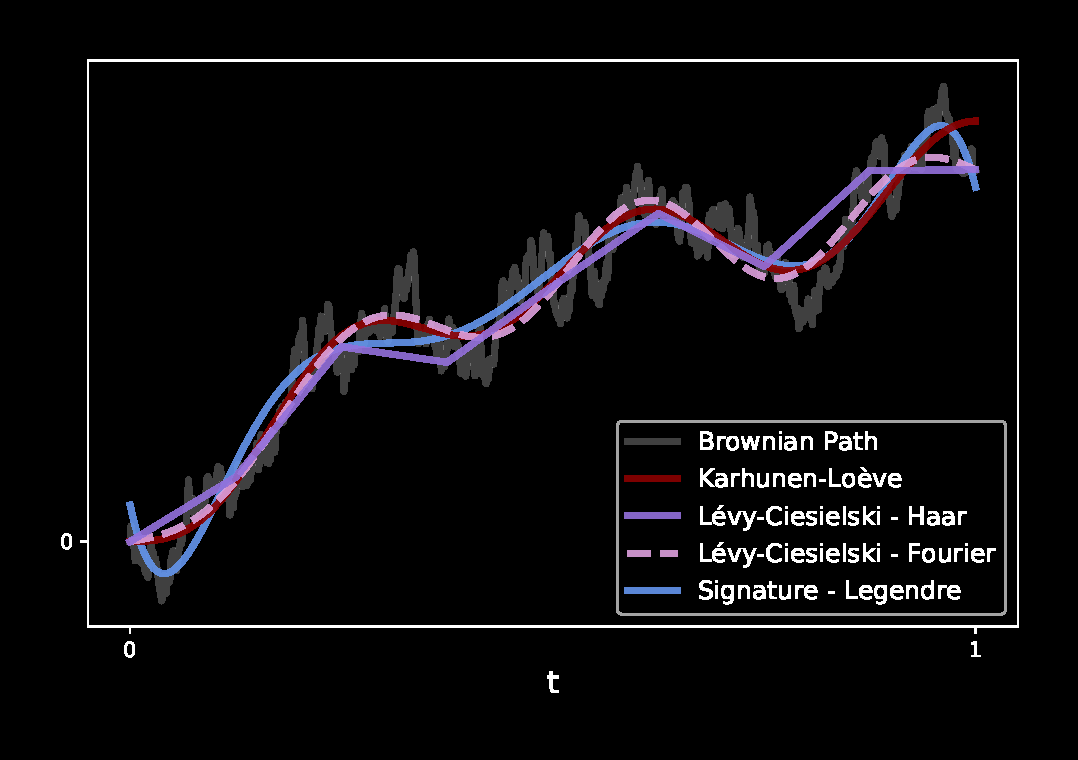
\includegraphics[scale = 0.45
    ]{KL/Figures/ProjPath.pdf}
    \label{fig:projPath}
\end{figure}